%-------------------------------------------------%
\subsection{Modelo: Clusters}
%-------------------------------------------------%

Se utilizarán técnicas de clusters sobre la base del tablón con el objetivo de observar si realmente existen agrupamientos basados en las características que contiene el tablón. Al terminar, se ingresará el clase sobre cada individuo y se analizará la composición de cada agrupamiento si se corresponde con dicho target. \\

\paragraph{\textbf{Criterio:}}

Como son solamente 2 las variables categóricas (EsTecnico y
sexo), en vez de calcular las distancias numéricas por un lado
(euclídea, manhattan, correlación, etc), las distancias categóricas por
otras (SMC, Jaccard, etc) y tratar de transformar esas matrices de
distancias en una nueva matriz unificada con criterios, se decide
transformar los datos categóricos en numéricos aprovechando que ambos
campos tiene solamente 2 valores por lo que estarán en los extremos
tomando una normalización entre 0 y 1. En el caso de las observaciones con valor nulo en la variable EsTecnico, se imputará con el valor
0.5 (mitad entre extremos)

\paragraph{Análisis de tendencia al agrupamiento}

El estadístico de Hopkins sobre el tablón original transformando las 2
variable categóricas en numéricas da 0.8893004. Es un valor cercano a 1
por lo que tiene mucha tendencia a ser clusterizado.

%-------------------------------------------------%
\subsubsection{\textbf{Determinar parámetros del modelo}}
%-------------------------------------------------%

\paragraph{\textbf{Matriz de Distancias de observaciones:}} euclideana

\paragraph{\textbf{Número óptimo de clusters}} \label{estudio-del-numero-optimo-de-clusters}
Para este estudio, se aplicaron 2 técnicas de agrupamiento llamadas kmeans y jerárquico. Se han calculado distintas métricas de agrupamiento y conectividad para determinar cual es el número óptimo de clusters, tomando como inicio 2 grupos y máximo 8.\\

Los resultados que se obtuvieron pueden observarse en: \ref{fig:kmeans_numoptimal_silhouette},  \ref{fig:kmeans_numoptimal_sumsquare} y \ref{kmeas_jerarquico_numoptimal}

\begin{figure}[!htb]
	\centering
	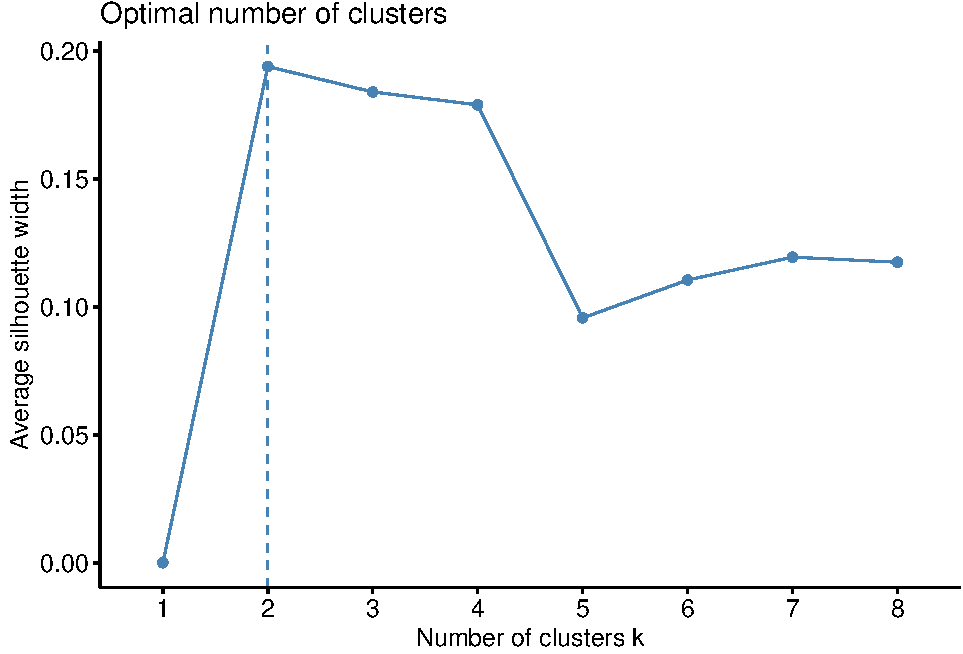
\includegraphics{imagenes/modelo_clusters/unnamed-chunk-15-1.pdf}
	%\includegraphics[width=0.25\textwidth]{mesh}
	\caption{Técnica Kmeans, Número óptimo de clusers, Criterio Silhouette}
	\label{fig:kmeans_numoptimal_silhouette}
\end{figure}

\begin{figure}[!htb]
	\centering
	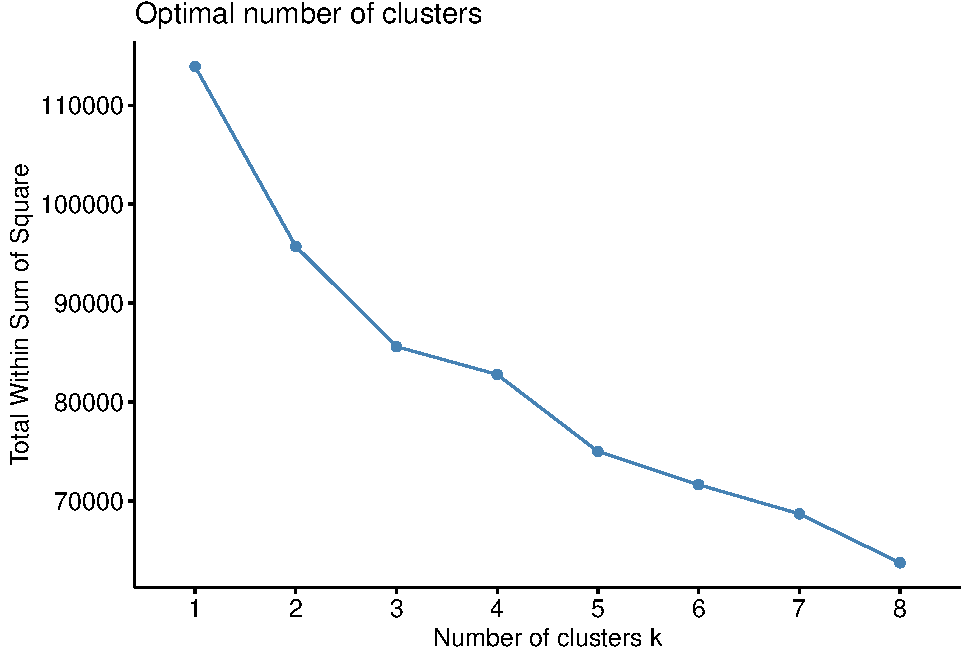
\includegraphics{imagenes/modelo_clusters/unnamed-chunk-15-2.pdf}
	%\includegraphics[width=0.25\textwidth]{mesh}
	\caption{Técnica Kmeans, Número óptimo de clusers, Criterio Suma de Cuadrados}
	\label{fig:kmeans_numoptimal_sumsquare}
\end{figure}

\clearpage



KMEANS y JERÁRQUICO analítico:\label{kmeas_jerarquico_numoptimal}

\begin{lstlisting}
## 
## Clustering Methods:
##  kmeans hierarchical 
## 
## Cluster sizes:
##  2 3 4 5 
## 
## Validation Measures:
##                                    2         3         4         5
##                                                                   
## kmeans       Connectivity     0.0000    3.1667  730.2742 1316.3881
##              Dunn             0.4693    0.5735    0.0471    0.0345
##              Silhouette       0.5937    0.5336    0.2070    0.1796
## hierarchical Connectivity     3.1667    3.1667    9.2357   12.1647
##              Dunn             0.5713    0.5735    0.2744    0.2744
##              Silhouette       0.7329    0.5336    0.5198    0.4879
## 
## Optimal Scores:
## 
##              Score  Method       Clusters
## Connectivity 0.0000 kmeans       2       
## Dunn         0.5735 kmeans       3       
## Silhouette   0.7329 hierarchical 2
\end{lstlisting}

\begin{itemize}
	\item
	Método Kmeans: Los resultados anteriores de validaciones internas,
	coinciden en que la óptima solución son 2 clusters en las
	métricas de Siloutte y Connectivity mientras que para la métrica de
	Dunn el óptimo número de clusters sería 3.
	\item
	Método Jerárquico: En esta validación se agregó el método jerárquico en el cual las métricas Connectivity y Dunn dan resultados iguales 	mientras que en silhouette es mejor el resultado con 2 clusters.
\end{itemize}

\paragraph{\textbf{tipo de cluster jerárquico:}}
Se realizan 4 cluster jerarquicos, cada uno utilizando las medidas de distancias ``complete'', ``average'', ``single'', ``ward''. Se calcula el coeficiente de correlación cophenético y se elige el de mayor valor. La tabla comparativa puede observarse a continuación \ref{tab:tabla_cophenetic_jerarquico}. En este caso la mejor opción es ``average''. 

\begin{table}[!h]
	
	\caption{\label{tab:tabla_cophenetic_jerarquico}Coef. cophenetic por cada tipo de cluster jerárquico}
	\centering
	\begin{tabular}[t]{lr}
		\toprule
		\rowcolor{black}  \multicolumn{1}{c}{\textcolor{white}{\textbf{metodo}}} & \multicolumn{1}{c}{\textcolor{white}{\textbf{coeficiente\_cofenetico}}}\\
		\midrule
		\rowcolor{gray!6}  complete & 0.7199776\\
		average & 0.8142721\\
		\rowcolor{gray!6}  single & 0.7217462\\
		ward & 0.3765082\\
		\bottomrule
	\end{tabular}
\end{table}



\paragraph{\textbf{Conclusión General}}
La conclusión es que la mejor opción es hacer clusters de 2 grupos ya sea por el método Kmeans o Jerárquico.


%-------------------------------------------------%
\subsubsection{\textbf{Modelar}}
%-------------------------------------------------%

\paragraph{\underline{\textbf{Cluster Kmeans}}}\label{cluster-kmeans}

Tomando como referencia las validaciones anteriores, se realiza un
cluster kmeans con 2 centroides. Este método se repetirá 25 veces
distintas y se elegirá el mejor.\\
Dicho procedimiento arroja resultados \ref{fig:kmeans_cluster_optimo} y \ref{fig:kmeans_cluster_optimo_silhouette}.

\begin{figure}[!htb]
	\centering
	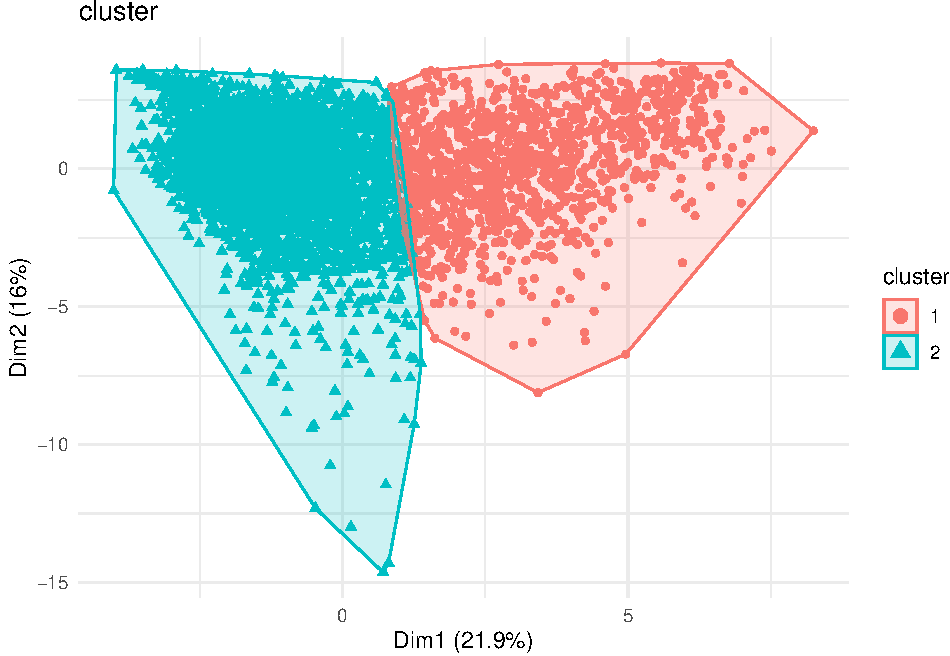
\includegraphics{imagenes/modelo_clusters/unnamed-chunk-18-1.pdf}
	%\includegraphics[width=0.25\textwidth]{mesh}
	\caption{Cluster óptimo Kmeans con 2 centroides. Variabilidad explicada 37.9\%}
	\label{fig:kmeans_cluster_optimo}
\end{figure}

\begin{figure}[!htb]
	\centering
	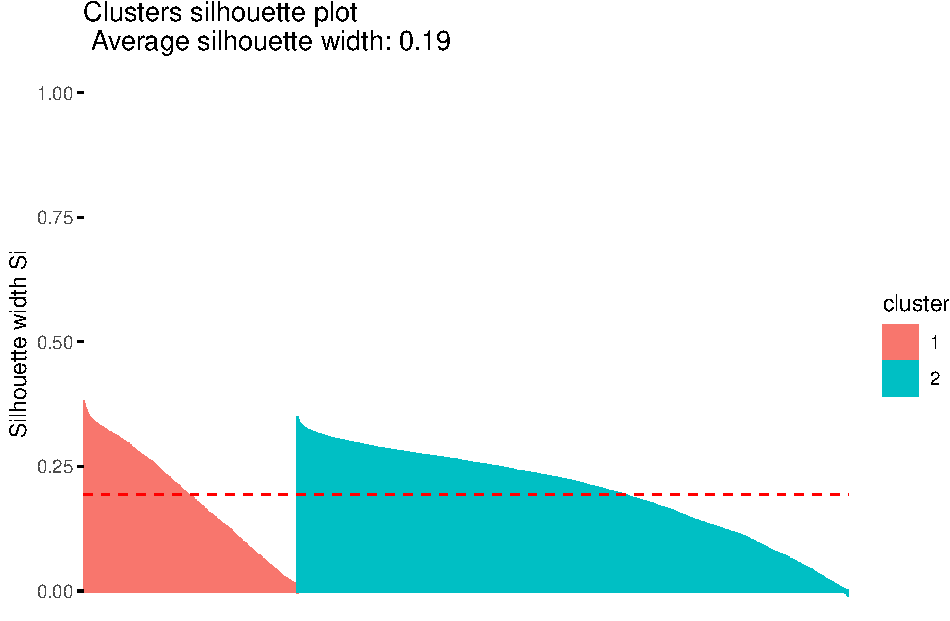
\includegraphics{imagenes/modelo_clusters/unnamed-chunk-18-2.pdf}
	%\includegraphics[width=0.25\textwidth]{mesh}
	\caption{Silhouette del cluster óptimo de kmeans \ref{fig:kmeans_cluster_optimo}}
	\label{fig:kmeans_cluster_optimo_silhouette}
\end{figure}


\clearpage


\hypertarget{cluster-jeruxe1rquico}{%
	\paragraph{\textbf{\underline{cluster jerárquico}}}\label{cluster-jeruxe1rquico}}
En este submodelo debido a la gran cantidad de observaciones, no podrá mostrarse el dendograma completo. Por lo tanto, el modelo se ejecuta y según lo sugerido en
las validaciones, se realiza el corte en 2 grupos. La composición puede observarse en la siguiente sección.


%-------------------------------------------------%
\subsubsection{\textbf{Describir el modelo}}
%-------------------------------------------------%

\paragraph{\textbf{Kmeans}}
El cluster kmeans modelado en la sección anterior parece ser muy bueno. Por lo tanto el próximo paso es saber en que cluster cae cada observación según su target para realizar una descripción de su composición según nuestra variable de interés.\\
La tabla \ref{tab:kmeans_2_resumen} y la figura \ref{fig:kmeans_cluster_optimo_composicion} resumen dicho análisis. Puede observarse que un grupo contiene solamente un 11,13\% de datos
erroneos, pero el otro grupo está muy balanceado. Por lo tanto, el
cluster de 2 grupos a pesar de que tenga muy buenos valores en las
validaciones realizadas, al verificar con el target real no da un buen resultado.

\begin{table}[!h]
	
	\caption{\label{tab:kmeans_2_resumen}Resumen composición de cluster Kmeans según clase desertor}
	\centering
	\resizebox{\linewidth}{!}{
	\begin{tabular}[t]{rrrrrr}
		\toprule
		\rowcolor{black}  \multicolumn{1}{c}{\textcolor{white}{\textbf{grupo}}} & \multicolumn{1}{c}{\textcolor{white}{\textbf{cant\_integrantes}}} & \multicolumn{1}{c}{\textcolor{white}{\textbf{cant\_desertores}}} & \multicolumn{1}{c}{\textcolor{white}{\textbf{cant\_desertores\_pct}}} & \multicolumn{1}{c}{\textcolor{white}{\textbf{cant\_no\_desertores}}} & \multicolumn{1}{c}{\textcolor{white}{\textbf{cant\_no\_desertores\_pct}}}\\
		\midrule
		\rowcolor{gray!6}  1 & 1275 & 142 & 11.13725 & 1133 & 88.86275\\
		2 & 3283 & 1858 & 56.59458 & 1425 & 43.40542\\
		\bottomrule
	\end{tabular}}
\end{table}


\begin{figure}[!htb]
	\centering
	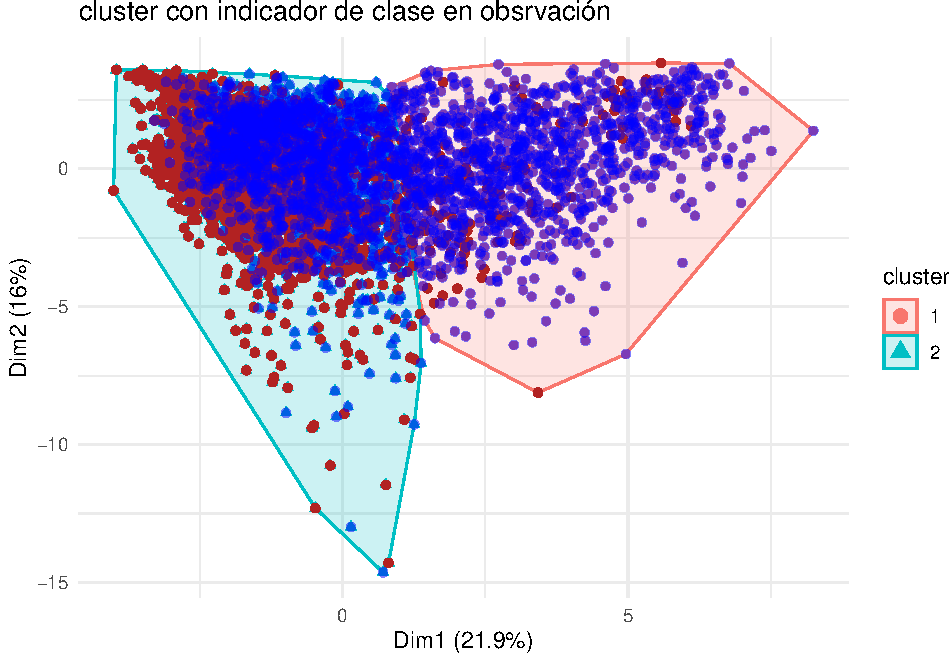
\includegraphics{imagenes/modelo_clusters/unnamed-chunk-21-1.pdf}
	%\includegraphics[width=0.25\textwidth]{mesh}
	\caption{Cluster óptimo Kmeans con 2 centroides. Variabilidad explicada 37.9\%. Indicación real de la clase}
	\label{fig:kmeans_cluster_optimo_composicion}
\end{figure}



\paragraph{\textbf{jerárquico}}

La composición de los grupos puede observarse en la tabla \ref{tab:tabla_jerarquico_composicion}. La misma detalla un grupo muy numeroso y otro muy chico y
ambos estan muy mezclados en función el target. Por lo tanto, el método
jerárquico no es adecuado.

\begin{table}[!h]
	
	\caption{\label{tab:tabla_jerarquico_composicion}Composición de clusters según la clase deserto}
	\centering
	\resizebox{\linewidth}{!}{
		\begin{tabular}[t]{rrrrrr}
			\toprule
			\rowcolor{black}  \multicolumn{1}{c}{\textcolor{white}{\textbf{grupo}}} & \multicolumn{1}{c}{\textcolor{white}{\textbf{cant\_integrantes}}} & \multicolumn{1}{c}{\textcolor{white}{\textbf{cant\_desertores}}} & \multicolumn{1}{c}{\textcolor{white}{\textbf{cant\_desertores\_pct}}} & \multicolumn{1}{c}{\textcolor{white}{\textbf{cant\_no\_desertores}}} & \multicolumn{1}{c}{\textcolor{white}{\textbf{cant\_no\_desertores\_pct}}}\\
			\midrule
			\rowcolor{gray!6}  1 & 4550 & 1996 & 43.86813 & 2554 & 56.13187\\
			2 & 8 & 4 & 50.00000 & 4 & 50.00000\\
			\bottomrule
	\end{tabular}}
\end{table}


\subsubsection{\textbf{Extensión de Clusters}}

A pesar del estudio de validaciones y resultados anteriormente,
se propone realizar varios modelos de cluster cambiando métodos y cantidad de grupos formados para estudiar los resultados. \\
De esta forma se pretende evaluar si existe algún modelo que sin importar la cantidad de grupos, represente mayoritariamente a las observaciones que lo componen según la clase deserto, la cual no es incluida para realizar los clusters.\\
La hipótesis es que como los resultados reales hacen referencia al target,
campo que no se incluye en los datos para hacer cluster al ser no
supervisado, podría darse el caso de que en la situación real otro
número de cluster sea óptima a la que arrojan las validaciones
matemáticas.\\

La tabla \ref{tab:tabla_muchos_clusters} y la figura \ref{fig:muchos_clusters} detallan los resultados de este experimento. La figura muestra la misma información que el cuadro anterior. En el eje
x indica que tipo de cluster es, cuantos clusters y la clase deserto
(``S'' y ``N''). En el eje y se indica el numero de cluster, por lo que
los cluster armados solo con 2 grupos, habrá información únicamente
hasta esa altura. Por ejemplo, para el caso de aplicar un método
jerárquico de 2 clusters podemos observar que en el primer cluster
tenemos 2554 casos Negatigos y 1996 casos positivos, mientras que el
cluster número 2 está conformado de 4 casos negativos y 4 casos
positivos.


\begin{table}[!h]
	
	\caption{\label{tab:tabla_muchos_clusters}Resumen por tipo de cluster, cantidad de clusters y la composición de cada uno según la clase deserto}
	\centering
	\resizebox{\linewidth}{!}{
		\begin{tabular}[t]{lrrrrrrrrrrr}
			\toprule
			\rowcolor{black}  \multicolumn{1}{c}{\textcolor{white}{\textbf{metodo}}} & \multicolumn{1}{c}{\textcolor{white}{\textbf{numero\_clusters}}} & \multicolumn{1}{c}{\textcolor{white}{\textbf{1\_N}}} & \multicolumn{1}{c}{\textcolor{white}{\textbf{1\_S}}} & \multicolumn{1}{c}{\textcolor{white}{\textbf{2\_N}}} & \multicolumn{1}{c}{\textcolor{white}{\textbf{2\_S}}} & \multicolumn{1}{c}{\textcolor{white}{\textbf{3\_N}}} & \multicolumn{1}{c}{\textcolor{white}{\textbf{3\_S}}} & \multicolumn{1}{c}{\textcolor{white}{\textbf{4\_N}}} & \multicolumn{1}{c}{\textcolor{white}{\textbf{4\_S}}} & \multicolumn{1}{c}{\textcolor{white}{\textbf{5\_N}}} & \multicolumn{1}{c}{\textcolor{white}{\textbf{5\_S}}}\\
			\midrule
			\rowcolor{gray!6}  jerarquico & 2 & 2554 & 1996 & 4 & 4 & NA & NA & NA & NA & NA & NA\\
			jerarquico & 3 & 2544 & 1972 & 10 & 24 & 4 & 4 & NA & NA & NA & NA\\
			\rowcolor{gray!6}  jerarquico & 4 & 2544 & 1970 & NA & 2 & 10 & 24 & 4 & 4 & NA & NA\\
			jerarquico & 5 & 2543 & 1970 & NA & 2 & 10 & 24 & 1 & NA & 4 & 4\\
			\rowcolor{gray!6}  kmeans & 2 & 1133 & 142 & 1425 & 1858 & NA & NA & NA & NA & NA & NA\\
			\addlinespace
			kmeans & 3 & 878 & 82 & 611 & 604 & 1069 & 1314 & NA & NA & NA & NA\\
			\rowcolor{gray!6}  kmeans & 4 & 1028 & 1252 & 842 & 73 & 14 & 28 & 674 & 647 & NA & NA\\
			kmeans & 5 & 725 & 576 & 400 & 837 & 606 & 487 & 14 & 28 & 813 & 72\\
			\bottomrule
	\end{tabular}}
\end{table}


\begin{figure}[!htb]
	\centering
	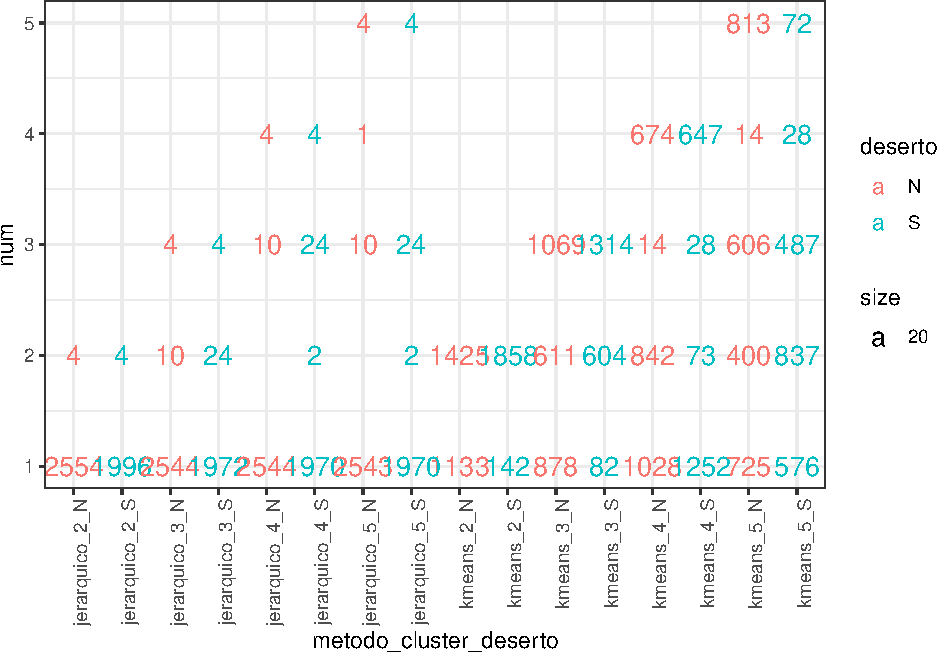
\includegraphics{imagenes/modelo_clusters/unnamed-chunk-25-1.pdf}
	%\includegraphics[width=0.25\textwidth]{mesh}
	\caption{Composición de muchos clusters distintos según target}
	\label{fig:muchos_clusters}
\end{figure}


\paragraph{\textbf{Conclusión general}}
la conclusión general es que ninguna de las variantes analizadas en este grid de clusters aún cambiando parámetro y métodos logra una identificación de grupos o subgrupos pertenecientes a alguna de las dos clases reales que hacen referencia a la deserción.\\





